\documentclass{article}

\usepackage{graphicx}
\usepackage{amsmath}
\usepackage{siunitx}
\usepackage{placeins}

\usepackage[margin=1in]{geometry}
\usepackage{float}


\def\hwtitle{Computational Physics HW7}
\def\hwauthor{Ethan Rooney}
\def\hwdate{2020-04-01}

\usepackage{fancyhdr}
\lhead{\hwauthor}
\chead{\hwtitle}
\rhead{\hwdate}
\lfoot{\hwauthor}
\cfoot{}
\rfoot{\thepage}
\renewcommand{\footrulewidth}{0.4pt}
\pagestyle{fancy}

\author{\hwauthor}
\title{\hwtitle}
\date{\hwdate}

\begin{document}

\maketitle
\thispagestyle{fancy}

\section{Introduction}
 
 Bootstrapping is a powerful technique providing us with a way to get an understanding of the underlying distribution in a sample of data.

\section{Results}

\subsection{Question 1}

See below the distribution of \texttt{drand48} and \texttt{gausrand}. These methods produce a reasonably good approximate distributions. There is high agreement between the PDF and the Histogram.

\begin{figure}[!htb]
	\begin{center}
		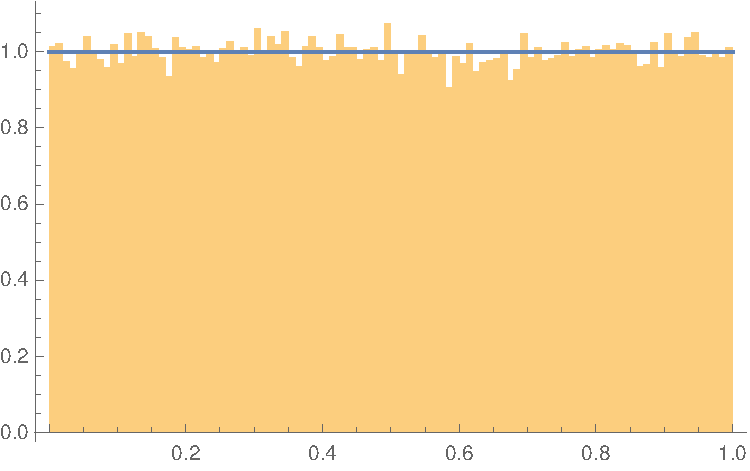
\includegraphics[width=0.6\textwidth]{p1a.pdf}
	\end{center}
	\caption{The PDF for a random number between 0 and 1 being chosen VS the Distribution of numbers generated by \texttt{drand48}}
\label{fig:qual}
\end{figure}
\FloatBarrier

\begin{figure}[!htb]
	\begin{center}
		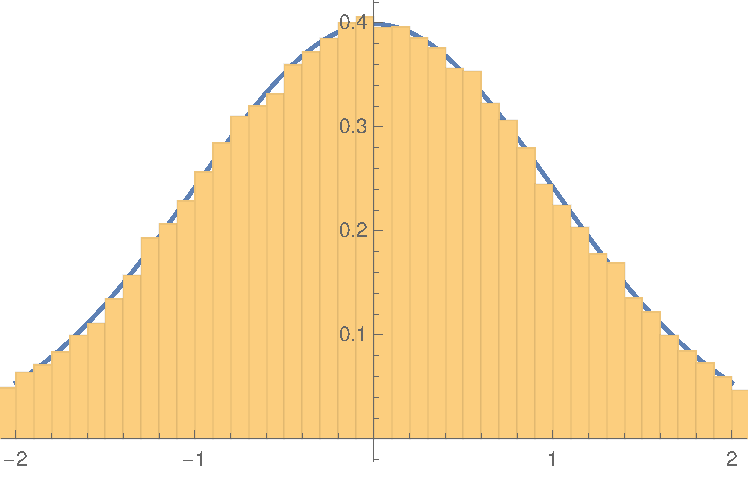
\includegraphics[width=0.6\textwidth]{p1b.pdf}
	\end{center}
	\caption{The PDF for a random number between 0 and 1 being chosen VS the Distribution of numbers generated by \texttt{gausrand}}
\label{fig:qual}
\end{figure}
\FloatBarrier

\subsection{Question 2}

When using the \texttt{gausrand} to generate 100,000 products of $x\times y$ with $\overline{x}=1,\sigma_x=2$ and $\overline{y}=4,\sigma_y=1$ we get the Histogram seen below. When compared to the PDF we see that the peak is higher than the naive approach.

\begin{figure}[!htb]
	\begin{center}
		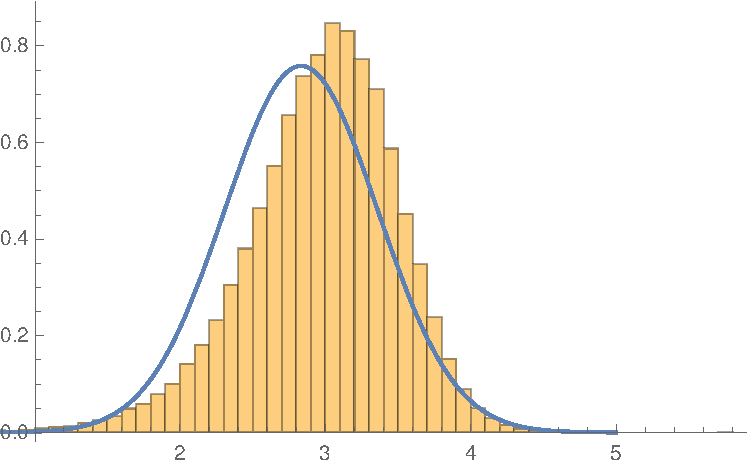
\includegraphics[width=0.6\textwidth]{p2a.pdf}
	\end{center}
	\caption{The histogram of the result of $x\times y$ with $\overline{x}=1,\sigma_x=2$ and $\overline{y}=4,\sigma_y=1$ vs PDF}
\label{fig:qual}
\end{figure}
\FloatBarrier

\subsection{Question 3}

\begin{figure}[!htb]
	\begin{center}
		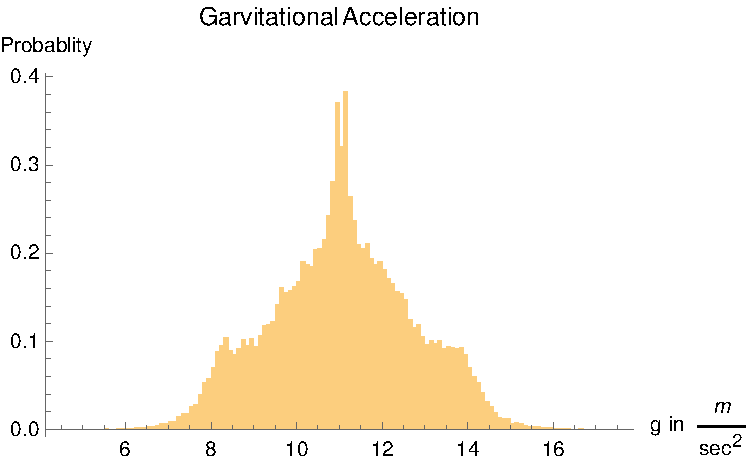
\includegraphics[width=0.6\textwidth]{p3a.pdf}
	\end{center}
	\caption{Results of 100000 bootstraps of cannonball.dat}
\label{fig:qual}
\end{figure}
\FloatBarrier

When using \texttt{gausrand} to generate 100000 values of $g$ we find  $g = 11 \pm 1.66 \frac{m}{s^2}$ to 1 standard deviation which to the accuracy of this dataset is a correct value of $g$ when compared to the canonical value of  $g=9.8 \frac{m}{s^2}$

\subsection{Question 4}

This question is confusingly worded and requests actions which cannot be performed in Mathematica. I petition it should be turned into a bonus question.

\subsubsection{Task 1}

\begin{center}
	\begin{tabular}{ |c|c|c| }
		\hline
		$t$ &  $y_t$ &  $\sigma_y$\\
		0.0 & 16381.3 & 101.903 \\
		0.5 & 16380.9 & 101.563 \\
		1.0 & 16377.6 & 102.517 \\
		1.5 & 16371.3 & 101.983 \\
		2.0 & 16364.3 & 101.296 \\
		2.5 & 16352.6 & 103.330 \\
		3.0 & 16340.3 & 102.216 \\
		3.5 & 16324.6 & 102.911 \\
		4.0 & 16306.0 & 101.821 \\
		4.5 & 16286.1 & 102.012 \\
		5.0 & 16263.0 & 101.756 \\
		5.5 & 16237.9 & 101.967 \\
		6.0 & 16210.1 & 102.882 \\
		\hline
	\end{tabular}
\end{center}

I did the first part, however \texttt{ErrorListPlot} does not exist as a function in Mathematica.

\subsubsection{Task 2}

Not sure what this section was asking for. So I made a histogram of what the distribution would look like if you generated Gaussian random values of $y_i$ and put it into a $\chi^2$ fitter 100000 times.

\begin{figure}[!htb]
	\begin{center}
		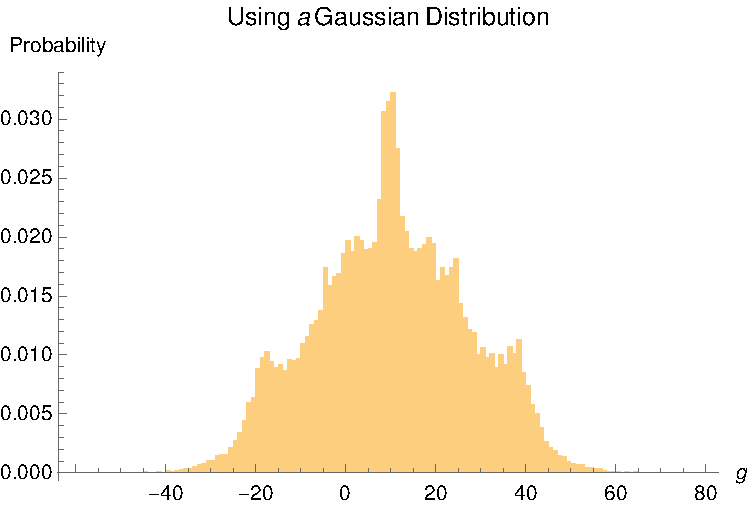
\includegraphics[width=0.6\textwidth]{p4t2a.pdf}
	\end{center}
	\caption{Results of 100000 gausrand of cannonball.dat}
\label{fig:qual}
\end{figure}
\FloatBarrier

We get a mean value of $g=9.83 \frac{m}{s^2}$ with a $\sigma_g = 17.6 \frac{m}{s^2}$ 

\subsubsection{Task 3}

I am not sure how this is different from Task 2, So instead I am just going to print the bootstrapped output of the $\chi^2$ fitters output for g. 


\begin{figure}[!htb]
	\begin{center}
		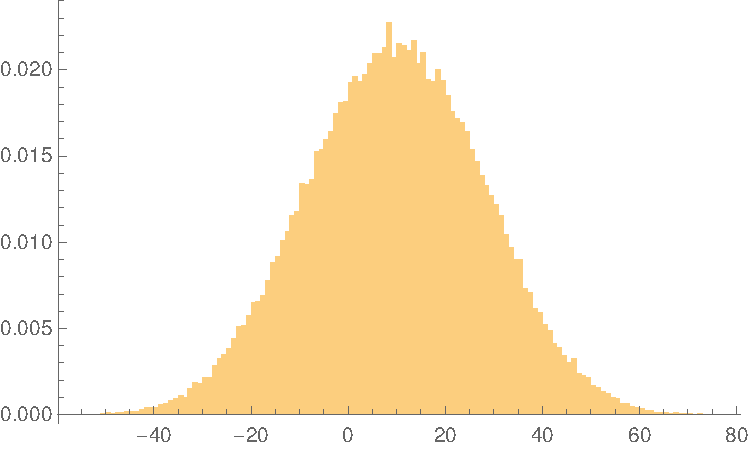
\includegraphics[width=0.6\textwidth]{p4t3a.pdf}
	\end{center}
	\caption{Results of 100000 bootstraps of bootstrap.dat}
\label{fig:qual}
\end{figure}
\FloatBarrier

Here we get $ g= 9.7 \frac{m}{s^2}$ with a $\sigma_g = 18.1 \frac{m}{s^2}$

The values of g are consistent with each other, but you van see from the histogram bootstrapping provides a more consistent normal distribution.


\section{Conclusion}

The homework was very confusing especially the difference between the tasks\ldots I essentially just started guessing what was being asked of me. I would hope for some clarification to be added for future classes.

\end{document}

